\documentclass{article}
\usepackage{graphicx} % Required for inserting images
\usepackage{hyperref} % Required for hyperlinks
\usepackage{amsmath}
\graphicspath{ {./images/} }
\newcommand\tab[1][1cm]{\hspace*{#1}}
\title{Analyzing the Citation Rate of a Scientific Paper Using ML and Graph Algorithms}
\author{Vladimir Zakharov, Sergey Fedchin, Artem Chebykin}
\date{Fall 2024}

\begin{document}

\maketitle

\section{Introduction}

\subsection{Paper Overview}

\tab Citation rate is an important metric to know about a scientific paper. It is often referred to as a KPI for researchers. Governmental agencies and scientists pay attention to the citation rate, when evaluating the quality of the paper. Hence, it is important to understand what exactly affects the citation of your work. In our research, we investigate the connection between various properties of scientific papers and their citation rates, using machine learning and graph algorithms. \\

\subsection{Field Overview}
\tab There are quite a few different papers that focus on predicting the citation rate. Most of them use only simple ML methods to obtain results, while we focus more on implementing graph algorithms to perform this task. The studies we have analyzed are: \\

\tab \href{https://link.springer.com/chapter/10.1007/978-3-642-40319-4_2?fromPaywallRec=false}{Predicting High Impact Academic Papers Using Citation Network Features} , that focused primarily on the graph features of the network, disregarded any meta-information about the paper.\\

\tab \href{https://link.springer.com/article/10.1007/s11192-020-03479-5?fromPaywallRec=true}{Predicting the future success of scientific publications through social network and semantic analysis} on the other hand, took into account the semantic structure of papers. However, this study used graph information only to create vertex features (betweenness, degree, etc.)\\

\tab \href{https://link.springer.com/chapter/10.1007/978-3-319-06483-3_4?fromPaywallRec=true}{Learning to Measure Influence in a Scientific Social Network} considered not only the author of a publication but also their co-authors, thus creating a more informative structure; yet only simple ML methods were used to conduct the research.\\
\section{Data Acquisition and Preprocessing}

\tab	The amount of data and its quality is the basis for any data science research. To explore the dependencies between the paper citation rate and its inner properties, we have chosen the dataset: \href{https://www.kaggle.com/datasets/wolfram77/graphs-snap-cit}{HepTh dataset} .The dataset represents the scientific paper citation graph in the field of high-energy physics in the years 1991 to 2003 \\
\tab	 An oriented edge between vertices a$\rightarrow$b shows, that paper a cites paper b. Apart from the graph information itself, we are also provided with various features of each paper, which are, however, not standardized. Some features only appear in few papers, while others are present for each. We have decided to keep and work with the following features present for each paper: date of publication, authors, title + abstract. \\
\tab	The task of processing the dates was particularly tricky one since that part of the data was stored in a multitude of different formats, and they had to be standardized. (We have chosen yyyy-mm-dd format for it). Furthermore, the graph included some edges that led from an older paper to a more recent one, which didn't make sense; hence, those edges were removed from our data. We have also transformed the list of authors from a string into an actual Python list and parsed the abstract from the metadata files provided in the dataset. \\
\tab	After all the described manipulations, the data was ready for further exploration and analysis. \\

\section{Exploratory Data Analysis}
\tab All calculations with the graph were performed using \href{https://networkx.org/}{NetworkX} library in Python because it has a well-written documentation and provides a convenient interface.
\subsection{General Properties}

\tab Let $V$ be the set of all papers (nodes) and $E = \{(v_1, v_2): v_1, v_2 \in V, v_1 \text{ cites } v_2 \}$ all the citations between papers (directed edges). Then $G(V, E)$ is our directed citation graph.
For this graph $$|V| = 27,376$$ $$|E| = 351,025$$
\tab The original graph had more nodes -- 27.7K, but we discovered that it had around 140 weakly connected components (connected components in graph $G'$ obtained from $G$ by disregarding the edges orientation). Most of them were of sizes 3-5 so we decided to leave only the main component and delete all the stray nodes. Due to the graph's nature, it cannot be strongly connected (and number of strongly connected components is exactly $|V|$), since strong connectivity means that there exists a path from any node $v$ to any other node $u$ in the component, but it yields a cycle, which is impossible in G, as stated earlier. \\
\tab Some graph properties are defined for directed graphs only if they are strongly connected: diameter --- length of the "longest shortest path", average path length, girth -- length of the smallest cycle (usually only defined for undirected graphs). What we can calculate is the density of $G$:
$$D(G) = \frac{|E|}{2\binom{|V|}{2}} \approx 0.00046,$$
so the graph is rather sparse, which makes sense if we take into account the nature of $G$.\\
\tab One other characteristic that we can compute is the average clustering coefficient, which is a measure of the degree to which nodes in a graph tend to cluster together. 
$$\bar{C}(G) = \frac{1}{n}\sum_{v \in V}C_v \approx 0.156,$$
where $C_v$ is the local clustering coefficient of the node $v$, defined as $$C_v = \frac{|E(G(N_v))|}{\binom{V(G(N_v))}{2}},$$
if $G(N_v)$ is the subgraph of $G$ with only the immediate neighbours of $v$  as nodes.

\subsection{Degree Distribution}
\tab One of the important aspects of any graph is the distribution of the degrees of nodes. Since our graph is directed, we will have 2 distributions: one for the in-degree (number of incoming edges) and one for the out-degree (number of outgoing edges).

\begin{figure}[h]
\centering
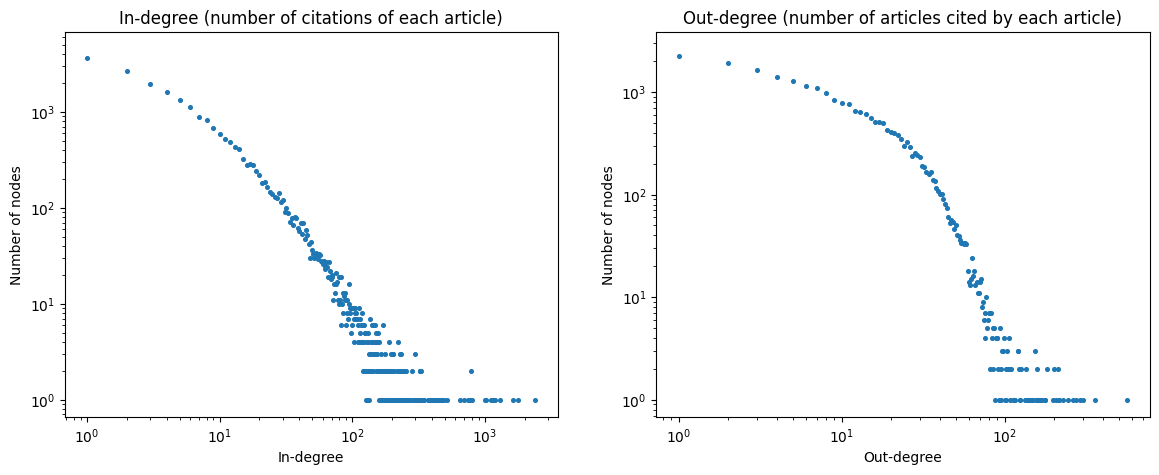
\includegraphics[width=1\linewidth]{degree_distribution.png}
\end{figure}
\newpage
The first distribution is rather typical for a scale-free network and follows the power law. However, it is not exactly the case with the out-degree distribution. The possible explanation to this is the following: if we look at the graph as a temporal graph (we have dates of each paper's publishing) out-degree of each node is determined on creation and does not change over time. In-degree, on the other hand, has a behaviour that is much closer to how degrees act in a usual social graph, developing over time.

\subsection{Centralities}
\tab Centralities are characteristics of nodes that determine how "important" or "popular" each of them is. There are several types of them and each measures this "importance" in its own way. We will visualize distribution of three centralities.
\begin{itemize}
\item[a)] Eigenvector centrality. In general, relative scores are assigned to all nodes in the network based on the concept that connections to high-scoring nodes contribute more to the score of the node in question than equal connections to low-scoring nodes.
\begin{figure}[h]
\centering
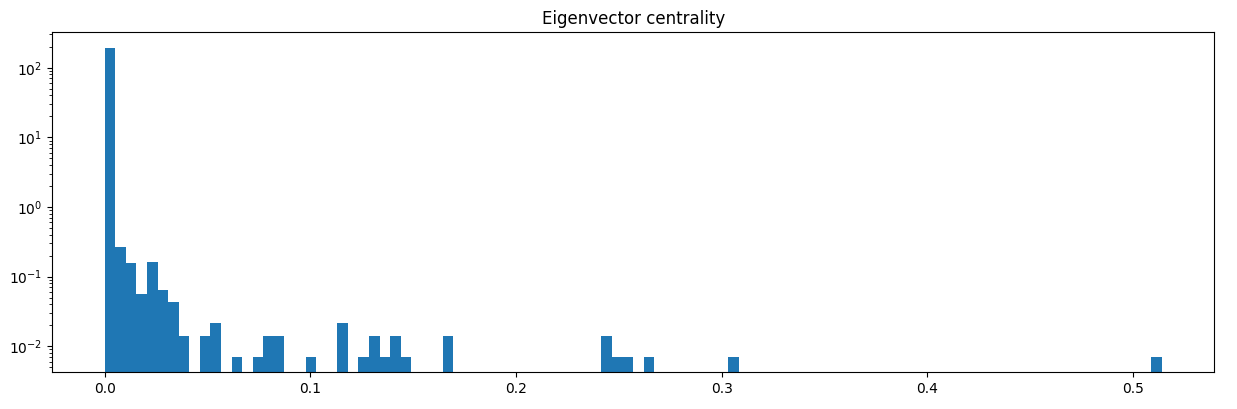
\includegraphics[width=1\linewidth]{centralities_eigenvector.png}
\end{figure}
\item[b)] Closeness centrality. It is calculated as the reciprocal of the sum of the length of the shortest paths between the node and all other nodes in the graph. It measures how "close" the node is to the rest of the graph.
\begin{figure}[h]
\centering
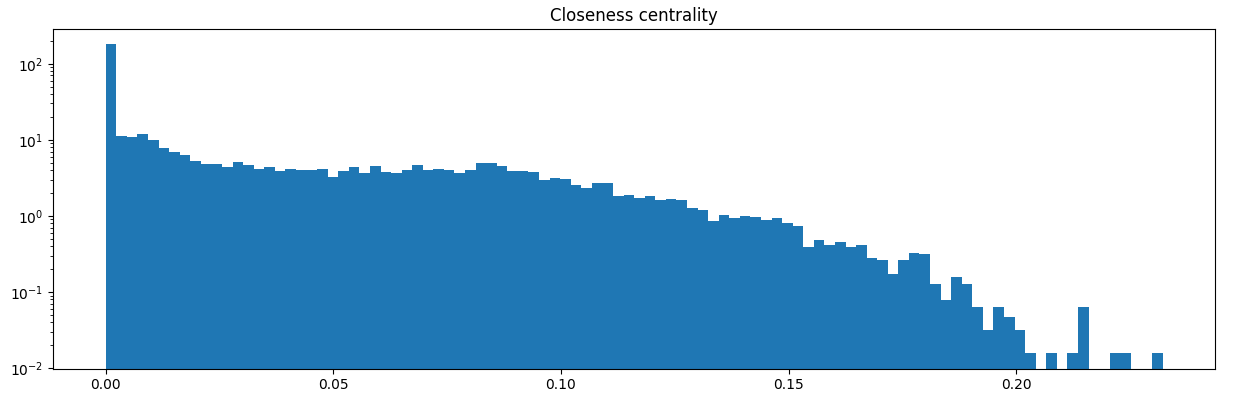
\includegraphics[width=1\linewidth]{centralities_closeness.png}
\end{figure}
\item[c)] Betweenness centrality. The betweenness centrality for each node is the number of shortest paths that pass through this node. In other words, it determines whether the node is a hub.
\begin{figure}[h]
\centering
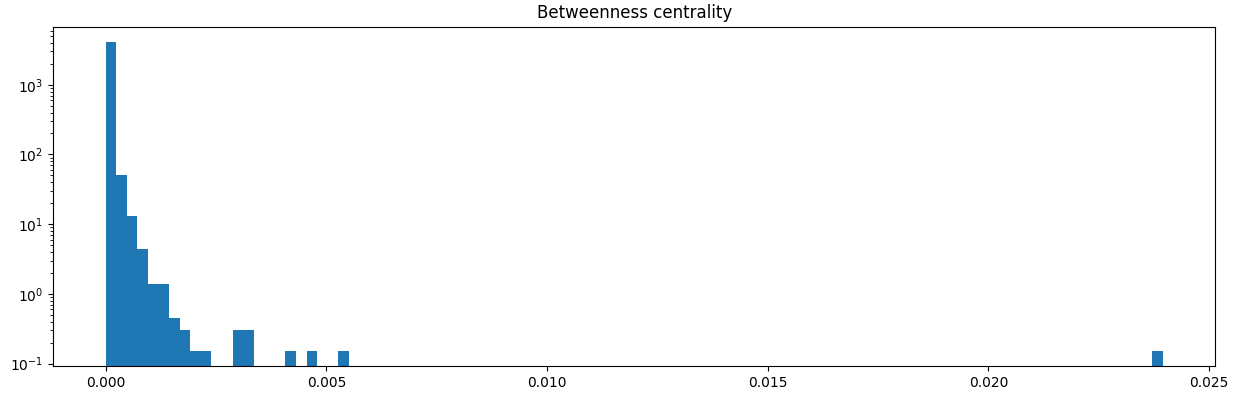
\includegraphics[width=1\linewidth]{centralities_betweenness.png}
\end{figure}
\end{itemize}

\subsection{Time Properties}
\tab Since our graph can be interpreted as a temporal graph, we can study the way its properties change over time. For instance, we discovered that the number of new papers per unit of time decreases:
\begin{figure}[h]
\centering
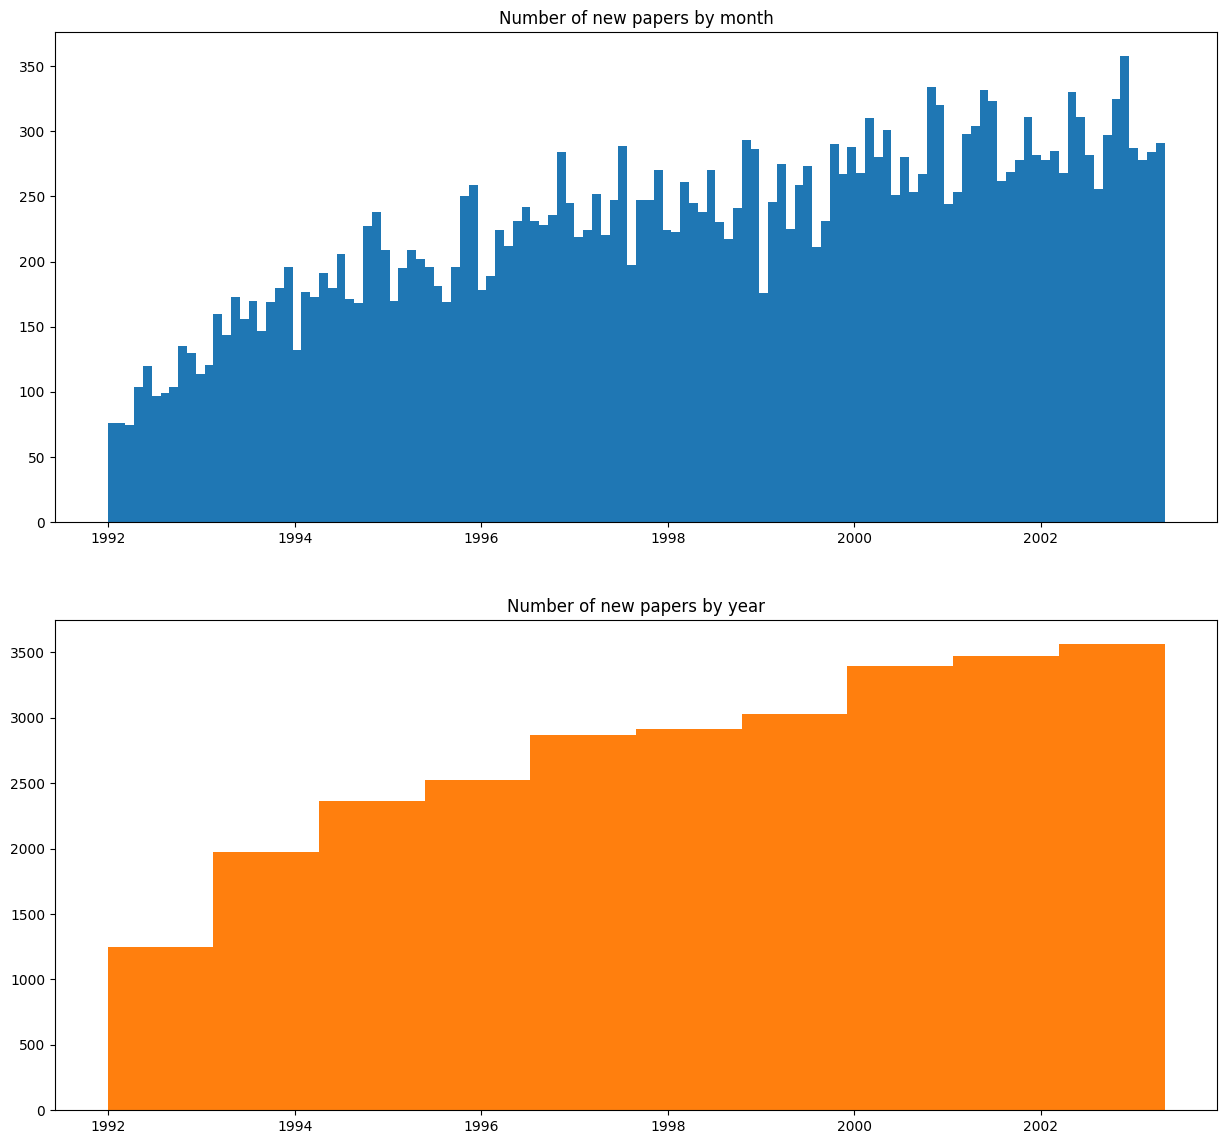
\includegraphics[width=0.9\linewidth]{new_papers_over_time.png}
\end{figure}
\newpage
Another interesting thing that we found is how average in-degrees and out-degrees change. This is the plot of average degrees in 2 months time from 1991 to 2003:
\begin{figure}[h]
\centering
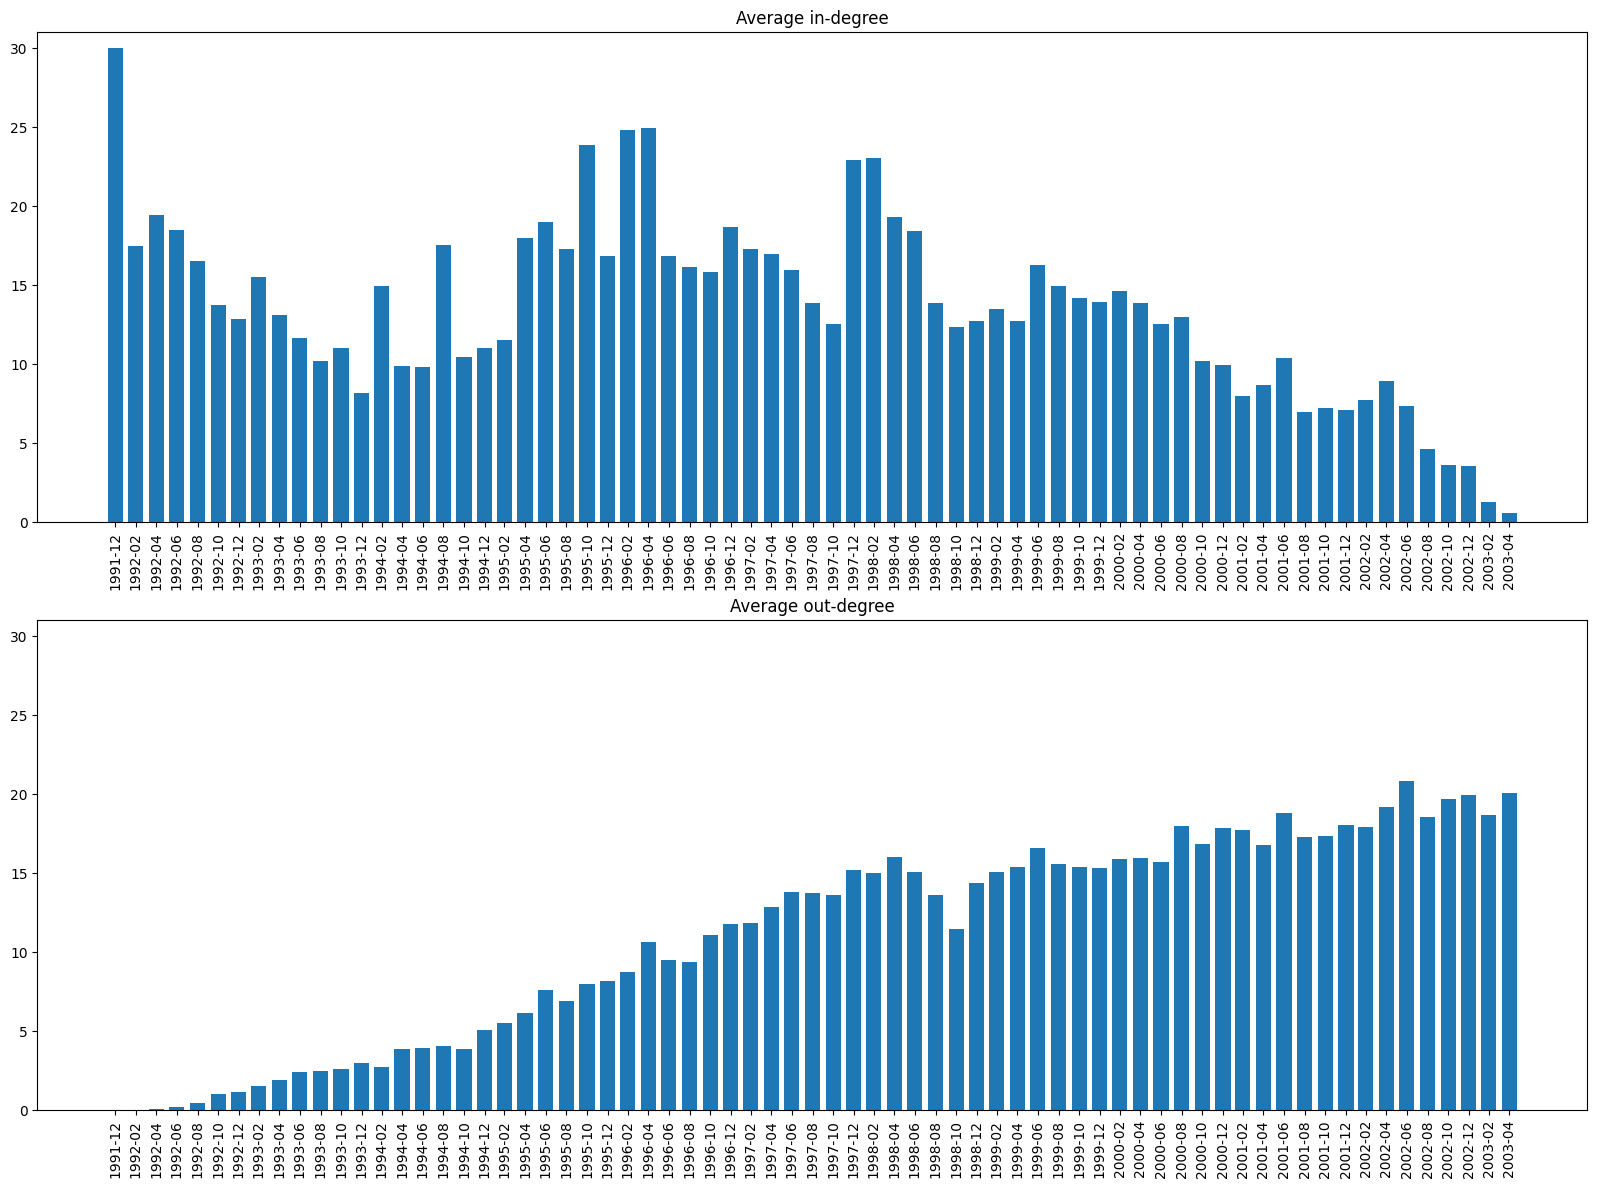
\includegraphics[width=1\linewidth]{degrees_over_time.png}
\end{figure}
A downwards trend in the end for in-degree and upwards trend in the beginning are noticeable. Explanation to this phenomena is rather simple: older papers had more time to gain popularity and therefore have more incoming edges, whereas papers from 2003 do not have any papers in our dataset that cite them. The opposite happens with the out-degree. Earlier papers cited even earlier papers (from 1980s) that were not included in our graph and thus have little to no outgoing edges. It is also worth noticing that the growth of out-degree slows down closer to 2003. It means that almost enough papers are included in the graph at that time to publish a paper sourcing only these modern papers in our dataset.
\subsection{Cluster properties}
We compared Louvain and label propagation community detection algorithms. All other methods were extremely slow. The best modularity was achieved by Louvain algorithm: 0.655 and 31 communities with fixed seed compared to 969 classes and 0.541 modularity using label propagation. We have divided the articles into the same number of clusters according to their abstracts using text embedding from `glove-wiki-gigaword-50` model (we averaged the embeddings of each word in the abstract) and KMeans algorithm. We also tried aglomerative clustering and gaussian mixture. Modularity for all of them was really poor, which is not suprising. That's the visualisation of it:
\begin{figure}[h]
\centering
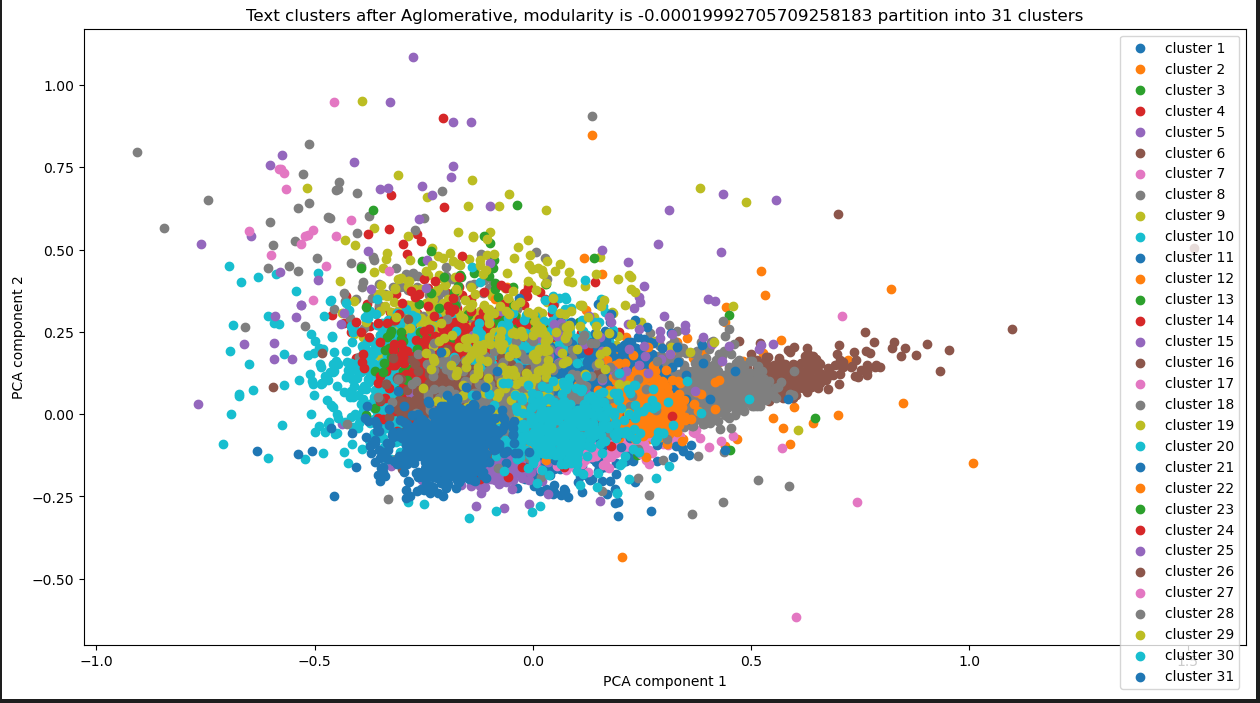
\includegraphics[width=1\linewidth]{Aglomerative.png}
\end{figure}
\begin{figure}[h]
\centering
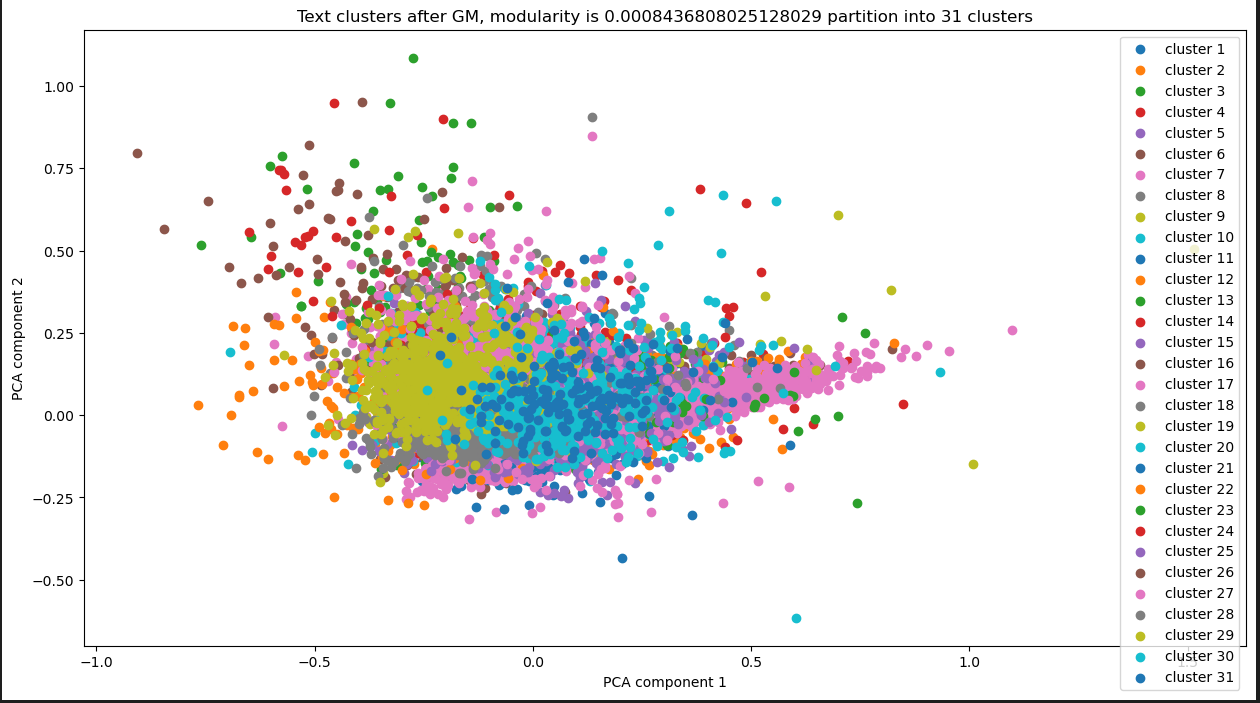
\includegraphics[width=1\linewidth]{gm.png}
\end{figure}
\end{document}